\documentclass[10pt,letterpaper]{article}
\usepackage[utf8x]{inputenc}
\usepackage{ucs}
\usepackage[english]{babel}
\usepackage{amsmath}
\usepackage{amsfonts}
\usepackage{amssymb}
\usepackage{amsthm}
\usepackage[left=3cm,right=3cm,top=3cm,bottom=3cm]{geometry}
\usepackage{graphicx}
\usepackage{color}
\usepackage{subcaption}
\usepackage{pdfpages}

\graphicspath{{img/}}

\newcommand{\pr}{{\normalfont \text{Pr}}}
\newcommand{\polylog}{{\normalfont \text{polylog}}}

\newtheorem{theorem}{Theorem}

\title{
	\textbf{CS552: Computer Networks\\
	Project Report}}

\author{Guido Tagliavini Ponce}

\begin{document}

\maketitle

\section*{Abstract}

We consider the paper ``Small Cache, Big Effect: Provable Load Balancing for Randomly Partitioned Cluster Services'' \cite{SmallCache}. In that paper it is shown, theoretically and empirically, that for a distributed key-value store randomly partitioned over $n$ back-end nodes, a front-end cache with $O(n \log n)$ items guarantees that no node will ever be overloaded. We take the most significant experiments and build a simulator to mimic them. Our results match the paper's to a great extent.

\tableofcontents

\section{Introduction}

In the paper ``Small Cache, Big Effect: Provable Load Balancing for Randomly Partitioned Cluster Services'' \cite{SmallCache} (from now on, \textit{the paper}), Fan et al. prove that given a key-value store (KVS) randomly partitioned across $n$ back-end servers, an $O(n \log n)$-size front-end cache is enough to guarantee that no adversary can overload a server. In other words, caching the $O(n \log n)$ most popular items is enough to guarantee load balance. This bound implies that only a small cache is needed, regardless of the number of items stored in the KVS or the access pattern.

Web services usually rely on front-end in-memory caches to reduce back-end servers' workload and hopefully balance the aggregate load \cite{Huang14}. Service designers can leverage the provable effectiveness of a small cache to work out service architectures that will meet, with high confidence, latency service-level agreements (SLAs). Moreover, it allows distributed KVS designers to bound the memory usage for caching purposes when resources are limited, for example when the cache is located in a network switch \cite{Li16}\cite{Jin17}.

\begin{figure}
\begin{center}	
	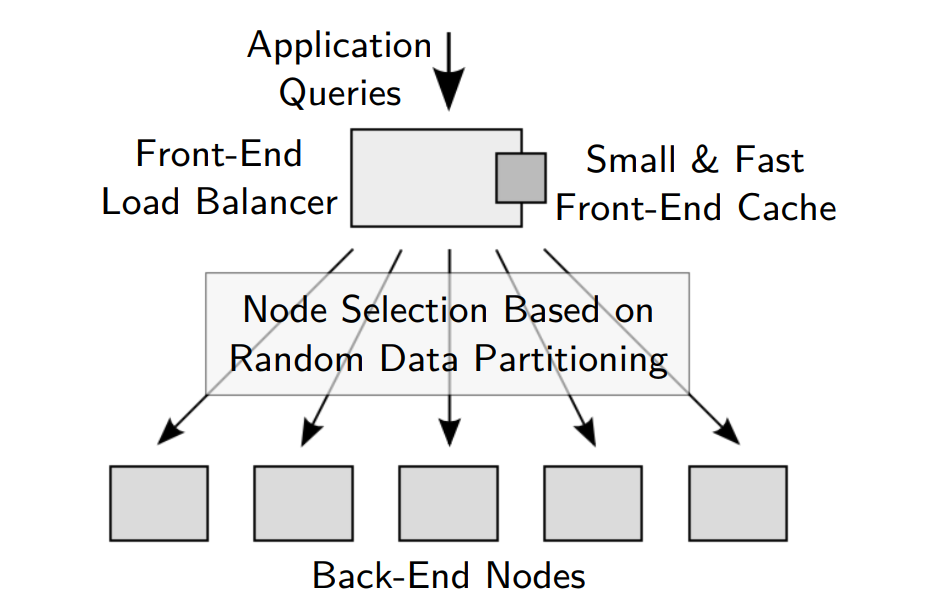
\includegraphics[scale=0.25]{kvs.png}
		\caption{A distributed KVS with a front-end cache.}
\end{center}
\end{figure}

Besides proving the theoretical bound, the authors validated their results by setting up a distributed KVS over $n = 85$ back-end nodes with a front-end cache stored on SRAM, and exposing the system to an adversarial workload. This type of workloads depend on the number of different keys that the adversary queries. We call this number the \textit{adversarial range}. The larger the adversarial range, the more spreaded the load. The authors perform several experiments, of which we are interested in three of them. They are presented in the following figures from the paper:

\begin{itemize}
	\item Figure 9, that shows the system-wide throughput as a function of the adversarial range, when there is no cache. The goal is to show that the system's performance with no cache can be terrible.
	\item Figure 11, that shows the system-wide throughput as a function of the cache size. For each cache size, several adversarial ranges are tested and the worst system performance is plotted. The goal is to find out what is the minimum cache size we need to guarantee full aggregate system throughput.
	\item Figure 10, that shows the system-wide throughput and back-end throughput as a function of the adversarial range, when there is an $\Theta(n \log n)$ cache. The goal is to show that an $\Theta(n \log n)$ cache effectively balances the load.
\end{itemize}

The goal of this project is to reproduce these measurements. The rest of this report is organized as follows. Is Section \ref{sec:caching} we explain why caching is a good load balancing technique. In Section \ref{sec:bound} we derive the $O(n \log n)$ bound proof. We describe the abstract model the authors use, which is useful to precisely understand what assumptions are made, and we discuss how these assumptions may limit the applicability of the bound. In Section \ref{sec:simulator} we describe the simulator we built to reproduce the experiments, and the challenges we faced during its development. Finally, in Section \ref{sec:results} we present our results and compare them against the paper's.

\section{Load balancing by means of caching}
\label{sec:caching}

Load balancing is an essential component of reliable web services. Query load is naturally imbalanced, because some of the items are more popular than others, and thus requested more frequently. It's also dynamic, since hot items change from time to time. A simple distributed KVS that uses a static assignment of items to machines, and does no effort to balance the load, will utterly fail to provide a good service because as soon as an item gets hot the machine that owns that item will get overloaded.

There are several load balancing techniques. Many of them are based on moving data around or replicating partitions. For example, Dean and Barroso \cite{Dean13} describe a set of techniques called \textit{micro-partitioning} and \textit{selective replication}, which consist of splitting the universe of key-values into small partitions, such that there are many more partitions than machines. Then, as load imbalance shows up, small hot partitions are moved from one machine to another to rebalance workload among all machines. On the downside, these kind of techniques are hard to engineer, and they incur on some network and space overhead.

Front-end caching is, in contrast, a much simpler load balancing technique. The basic idea is that items cached in a front-end node are retrieved much faster than queries that need to go to the back-end, thus alleviating back-end load. When an item is brought from the back-end, it is cached so that subsequent queries for that item are served instantly by the front-end. A typical web service can store several TB of data over the back-end nodes, so only a small fraction of the whole store can be cached in the front-end node.

Why is caching effective at load balancing? The key idea is that if there are only a few hot items, then the cache will answer all those requests, and as queries get spreaded over many items the load on individual back-end nodes gets diluted, so every server can keep up with the demand. Thus, the cache absorbs most of the work in the unbalanced scenario that hurts the back-end.

How big does the cache needs to be? We can assume the maximum query rate is bounded by the aggregate throughput of all back-end nodes, since beyond that threshold some node will necessarily get overloaded independently of how well the load is balanced. Since an adversary can put only a bounded load on the system, then for a sufficiently big adversarial range, the query rate per server will be small. The cache needs to be big enough so that if the adversary is able to bypass the cache, then by the time queries hit the back-end the maximum load on a single server is not too big.

\section{The $O(n \log n)$ bound}
\label{sec:bound}

\subsection{Model and assumptions}

We start defining some notation:

\begin{itemize}
	\item[] $n = $ \# of back-end nodes
	\item[] $m = $ \# of different keys stored
	\item[] $c = $ \# of items the cache can store
	\item[] $q = $ client query rate
	\item[] $t = $ maximum throughput of any back-end node
\end{itemize}

\noindent
Query rate and throughput are measured in QPS. The authors assume a system with the following properties:

\begin{enumerate}
	\item \textbf{Randomized key partitioning.} Each key is assigned to a random server, and this partitioning is unknown to clients.
	\item \textbf{Front-end is arbitrarily fast.} The front-end node is fast enough to handle an arbitrary number of queries per unit time, be it retrieving a cached item or forwarding a query to the back-end. Thus, the front-end is never a bottleneck.
	\item \textbf{Network is arbitrarily fast.} Network bandwidth and delay are never a bottleneck.
	\item \textbf{Perfect caching.} The cache knows what the $c$ most queried items will be, even before the sequence of requests starts.
	\item \textbf{Uniform cost.} The cost of processing a query is independent of the key and the back-end node serving the query.
\end{enumerate}

\noindent
The authors do not explicitly state the fast network assumption, but they mention it when they describe the experimental setting.

It's natural to ask is if these assumptions are reasonable. Randomized partitioning is realistic, since spreading the items uniformly is the most simple way to avoid imbalance, and it's what most distributed stores do. The front-end being arbitrarily fast is also reasonable, since a fast memory cache is able to perform hundreds of millions of lookups per second, enough to keep up with reasonably large demand rates. If the front-end turned into a bottleneck, we could add front-end nodes, and replicate the whole cache. This is feasible since, as we already advertised, only a small cache is necessary. The same reasoning holds for the arbitrarily fast network assumption. The uniform cost assumption is reasonable as well, because KVSs typically have similar access times for most of the keys.

In contrast, the perfect caching assumption is obviously unrealistic, since there is no such thing as an oracle that can tell us in advance which will the future requests be. The goal of this assumption is to simplify things enough to allow a theoretical analysis. However, the small cache argument extends, at least from a practical point of view, to real-life caches. To support this claim, we perform some experiments with an LRU cache.

We can outline the proof as follows:

\begin{enumerate}
	\item Bound the maximum query rate per key.
	\item Bound the expected number of maximum uncached queried keys on any server.
	\item The product of these two values yields a bound on the expected maximum load per machine. Since this bound is a function of $c$, we can choose $c$ such that the bound is below the capacity $t$ of every machine.
\end{enumerate}

\subsection{Optimal adversary}

The first step towards the bound is to devise an adversary that maximizes the chances of overloading some server. Let $q_{\max}$ be the maximum query rate going to some server. Our goal is to characterize an adversary that maximizes $E[q_{\max}]$. The bigger the $E[q_{\max}]$, the higher are the chances of overloading a server. In particular, if $E[q_{\max}] > t$, the adversary is expected to overload some server.

We assume that the adversary knows:
\begin{itemize}
	\item Which keys are stored in the system.
	\item The number of back-end servers $n$.
	\item The cache size $c$.
\end{itemize}

\noindent
However, we assume it doesn't know how the keys are hashed into the servers, and that it cannot learn this partitioning (i.e. it's not adaptive).

Number the keys from $1$ to $m$, and let $p_i$ be the probability that the adversary queries key $i$. That is, the adversary queries key $i$, $p_i$ of the time. Note that $p_1 + \dots + p_m = 1$. Assume, w.l.o.g., that $p_1 \geq p_2 \geq \dots \geq p_m$ (otherwise, reassign key numbers). Since the cache is perfect, it will contain keys $1, \dots, c$, at all times. Thus, for the adversary to maximize the expected $q_{\max}$, it should always prefer to query keys $c + 1, \dots, m$, and within this subset it should try to query as few keys as possible, as so to consolidate most of the load in as few servers as possible.

The key observation is that for any given key $1 \leq i < c$, the adversary doesn't benefit from querying $i$ more than $i + 1$. If so, we could subtract that difference from $p_i$ (the ranking $p_1 \geq \dots \geq p_m$ of keys by query frequency remains unchanged), and use that extra time to query uncached keys, increasing $q_{\max}$. This implies that $p_1 = \dots = p_c = h$ for some $h \in (0, 1)$. Thus, $p_i \leq h$ for every $i > c$. Since the optimal strategy is to put all the load in as few keys as possible, the adversary assigns probability $p_i = h$ for $i \geq c + 1$, while possible. Specifically, the adversary assigns probabilities $p_{c + 1} = \dots = p_{x - 1} = h$ and $p_x = 1 - (x - 1)h$, for some $x > c$. The value $x$ is the number of different keys queried by the adversary. The number $x$ is what we called the adversarial range. Figure \ref{fig:adversary} shows a picture of the strategy, which we took from the paper.

\begin{figure}
	\centering
	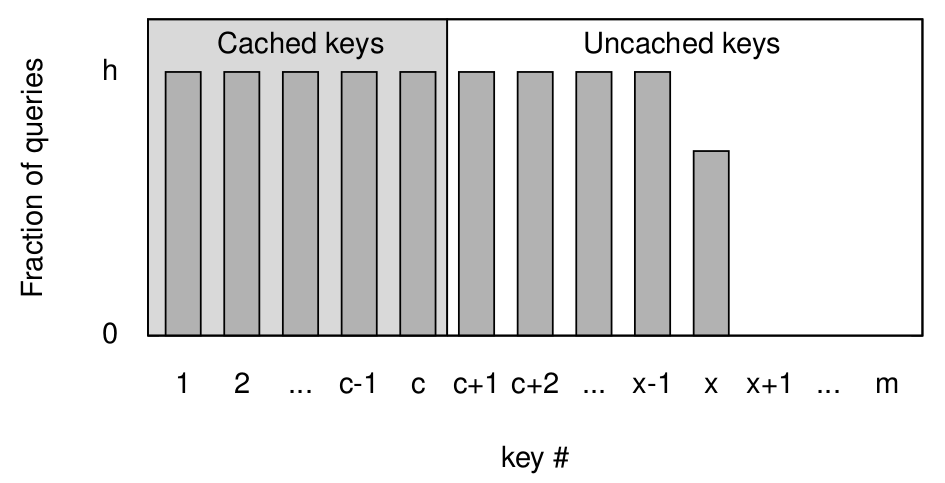
\includegraphics[scale=0.25]{img/adversary.png}
	\caption{Optimal adversarial strategy.}
	\label{fig:adversary}
\end{figure}

The important thing about this strategy is that it distributes the query frequency almost evenly over the adversarial range. More precisely, $h < 1 / (x - 1)$. We conclude that the maximum query rate per key is $hq < q / (x - 1)$.

\subsection{Key partitioning as a balls-into-bins game}

We can think the process of hashing keys into servers as randomly placing balls into bins. The maximum number of keys assigned to the same machine equals to the maximum number of balls in the same bin.

Balls-into-bins games are a well studied topic in probability theory, and it has many applications in computer science. In 1998, Raab and Steger \cite{Raab98} proved the following theorem, which provides an estimation on the maximum number of balls in a single bin.

\begin{theorem}[Restated Theorem 1 from \cite{Raab98}] Let $B$ be the random variable that counts the maximum number of balls in any bin, if we throw $M$ balls independently and uniformly at random into $N$ bins, with $N \log N \ll M \leq N \text{ }\polylog N$. Then,

\[\pr\left[B < \frac{M}{N} + \alpha \sqrt{2 \frac{M}{N} \log N}\right] = 1 - o(1)\]

\noindent
for any $\alpha > 1$.
\end{theorem}

The hypothesis $N \log N \ll M \leq N \text{ }\polylog N$ means that there should be a $\log$ factor more balls than bins, but at most a $\polylog$ factor. In the small cache paper, the authors use this bound in a context where the number of balls is certainly not bounded by $N \text{ } \polylog N$, because there are many more keys (usually millions) than a $\polylog$ factor of servers (usually tens or hundreds). The original theorem in \cite{Raab98} also states an estimation for the case $M \gg N \log^3 N$, which would be more adequate for our use case, but the authors didn't use it (presumably because it's more complex and thus harder to manipulate). However, they present evidence showing that the former estimation is still useful for this case (see Figure 4 in the paper).

In our case, we have $N = n$ bins, and $M = x - c$ balls, because we are only interested in counting uncached keys. Thus, by the previous theorem, the maximum number of queried keys in any server is bounded by

\[
\frac{x - c}{n} + \alpha \sqrt{2 \frac{x - c}{n} \log n}
\]

\noindent
for any $\alpha > 1$, w.h.p. Multiplying by the maximum query rate per key, we get

\begin{align*}
E[q_{\max}] &\leq \left(\frac{x - c}{n} + \alpha \sqrt{2 \frac{x - c}{n} \log n}\right) \frac{q}{x - 1}\\
&= \left(\frac{x - c}{x - 1} + \alpha \sqrt{2 \frac{x - c}{(x - 1)^2} n \log n}\right) \frac{q}{n}
\end{align*}

\noindent
If we maximize this expression as a function of $x$, we get

\begin{equation}
\label{eq:r_max}
E[q_{\max}] \leq \frac{1}{2}\left(1 + \sqrt{1 + 2\alpha^2\frac{n \log n}{c - 1}}\right)\frac{q}{n}
\end{equation}

\noindent
Thus, if we take $c = k n \log n + 1$, for some positive constant $k$, we get

\[
E[q_{\max}] \leq \left(\frac{1}{2} + \alpha\frac{\sqrt{2}}{2}\right) \frac{q}{n}
\]

\noindent
This means that the expected \textit{maximum} load per machine is at most a constant factor of the \textit{average} load per machine, implying that the overall load $q$ will be spreaded evenly among all $n$ servers. Since the aggregate back-end throughput must be $q$ or more, each machine should guarantee throughput $t \geq q / n$. Thus no machine will get more (than a small constant factor of the maximum) load than it can handle, in expectation. This concludes the proof of the bound.

Suppose $E[q_{\max}] = t$, which means that some machine is at maximum utilization but the system is not overloaded. Then, from Equation \ref{eq:r_max} we can derive the following lower bound on the maximum query rate tolerable by the system,

\begin{equation}
\label{eq:max_query_rate}
q \geq \frac{2nt}{\left(1 + \sqrt{1 + 2\alpha^2\frac{n \log n}{c - 1}}\right)}
\end{equation}

\section{The simulation}
\label{sec:simulator}

To reproduce the chosen set of experiments, we had to decide between simulating or emulating the system. Initially, we considered running an emulation of the distributed KVS system, using some network emulator software like Mininet, so as to replicate the system behavior as precisely as possible. It was soon clear that this was infeasible if we planned to run several back-end nodes, because they would all intensively contend with each other for the same machine resources. Too much contention could influence the measurements making them less reliable.

On the other hand, a simulation requires substantially less amount of resources at the cost of abstracting some features. Specifically, a simulation wouldn't execute real lookups on a store, and wouldn't send or receive queries through the network. Fortunately, these are not essential features, since cache effectiveness depends on the number of back-end nodes and how many QPS they can answer, but it doesn't matter what the lookup process is or what the answer is. Also, network communication between the client and the front-end, and between the front-end the servers, can be safely abstracted in since the distributed KVS built by the authors the line card bandwidth is high enough in every node so that network cost is a negligible part of the query latency. All in all, we decided that a simulation could accurately mimic the KVS.

\subsection{System specification}

The authors deployed the distributed store FAWN-KV \cite{Andersen09} with $n = 85$ back-end nodes. The front-end node uses a $10$GbE link and the back-end nodes use a $1$GbE link. The cluster stores $m = 8.5$M key-value pairs, each node responsible for $100$k of them. Back-end nodes serve queries at a rate of $t = 10000$QPS.

The client pipelines queries (i.e., sends one query after the other, without waiting for the answer) to hide network latency, but in order to keep the per-query latency under control it limits the maximum outstanding queries per back-end node to $1000$. When this value is reached, the client waits for the node's queue to empty, and then resends the query. The paper does not indicate the rate $q$ at which the client issues queries, but we can infer that for some experiments they used $q = nt$ (the aggregate throughput of all nodes), and for some others $q = 2nt$ (to stress the cache).

\subsection{Simulation design}

\paragraph{Overview}

The basic structure of our simulation is shown in Figure \ref{fig:simulator}. The main entities in the system are present as concrete objects of the simulation, and they interact in the expected way. These are the \texttt{client}, the \texttt{frontEndNode}, the \texttt{cache}, the \texttt{backEndNode}s and the \texttt{queue}s. The \texttt{queue} attached to each \texttt{backEndNode} contains all the pending queries for that node. When it reaches $1000$ queries, it rejects new requests. The rest of the objects are:

\begin{itemize}
	\item \texttt{simulator}: controls the simulation flow.
	\item \texttt{eventsQueue}: contains the events that will be executed next.
	\item \texttt{stats}: maintains statistics (like the number of queries issued so far) and how much time we have simulated.
\end{itemize}

\begin{figure}
	\centering
	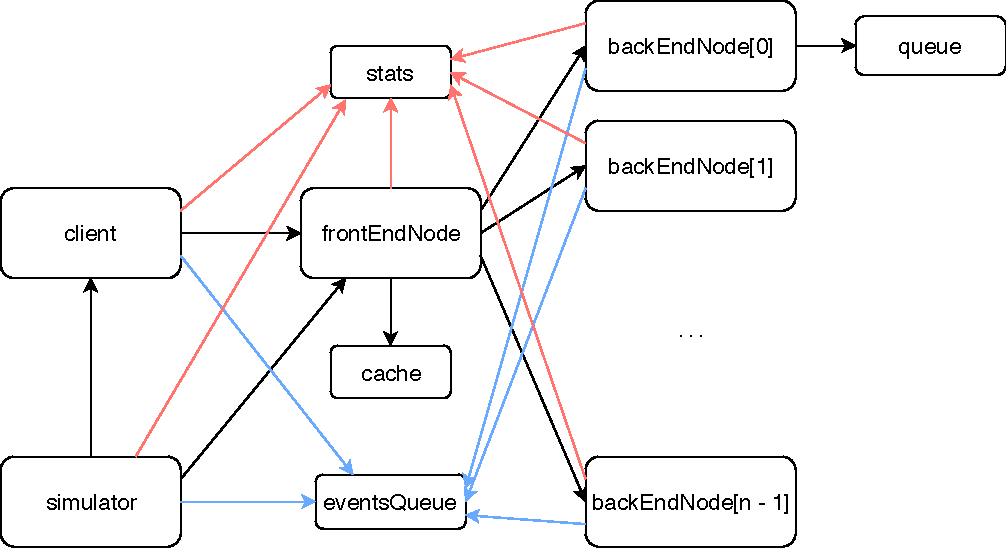
\includegraphics[scale=0.75]{img/simulator.pdf}
	\caption{Simplified object diagram of the simulator. Colors are just for clarity. Despite a single \texttt{queue} object is shown, every back-end node has one.}
	\label{fig:simulator}
\end{figure}

The basic idea is that events (e.g., the client issues a query) are triggered by the \texttt{simulator} the moment they are taken out from the \texttt{eventsQueue}. The events will be popped out in the order they should occur. To materialize this time ordering, we discretize the continuous into slots, each corresponding to some fixed amount of time, and each event is scheduled to happen at a specific time slot. There are three types of events:

\begin{itemize}
	\item \texttt{ClientSendNewQueryEvent}: when the client sends a new query.
	\item \texttt{ClientResendQueryEvent}: when a query that was rejected because a of a full queue, is now retried.
	\item \texttt{BackEndAnswerQueryEvent}: when a back-end server completes a key lookup.
\end{itemize}

\paragraph{Time discretization}

Let $\Delta$ be the amount of time that spans a single time slot. Since the client issues $q$ QPS and any back-end node answers $t$ QPS, we want $1 / q$ and $1 / t$ to be an integral multiple of $\Delta$. Since the adversarial query rate $q$ is usually set to a multiple of the server's throughput (e.g. $q = nt$ or $q = 2nt$), we can assume $q = st$ for some positive integer $s$. If we divide each second into $q$ slots, then $\Delta = 1 / q$, so a single slot is the time it takes to issue a query. Moreover, $s$ slots represent $s\Delta = s / q = 1 / t$ seconds, and thus $s$ slots are the time that takes a server to answer a query. Thus, this simple discretization works. In what follows, we will write $\texttt{slotsPerLookup} := s$.

\paragraph{Event execution}

The simulation can be described as a series of two-steps rounds. On each round, the \texttt{simulator} fetches the next event from the \texttt{eventsQueue}, and then executes it. This loop repeats until we have simulated as much time as desired.

When a \texttt{ClientSendNewQueryEvent} or \texttt{ClientResendQueryEvent} is executed, the \texttt{client} is called to send a query for a given key, and there are essentially three outcomes. In the event of a cache hit (Figure \ref{fig:query_hit}), the control goes back immediatly to the client, which schedules a \texttt{ClientSendNewQueryEvent} for the next time slot. If the item is not cached, there are two possibilities. If the target server's queue is not full (Figure \ref{fig:query_miss}), the query is enqueued and the control goes back to the client, which schedules the next \texttt{ClientSendNewQueryEvent}. Otherwise, if the queue is full (Figure \ref{fig:query_full_queue}), the client is informed the query has failed, and it schedules a \texttt{ClientResendQueryEvent} far enough in the future (after $1000$ back-end lookups) to retry when the queue is empty.

When a \texttt{BackEndAnswerQueryEvent} is executed (Figure \ref{fig:answer_query}), the corresponding \texttt{backEndNode} informs the \texttt{frontEndNode}, which in turn notices the cache. Upon learning about the new resolved query, and depending on the type of cache, the cache can decide to write-back the new item. In particular, perfect caches do not write-back, because they already have the hottest items, but our simplified implementation of an LRU cache does so.

\begin{figure}
	\centering
	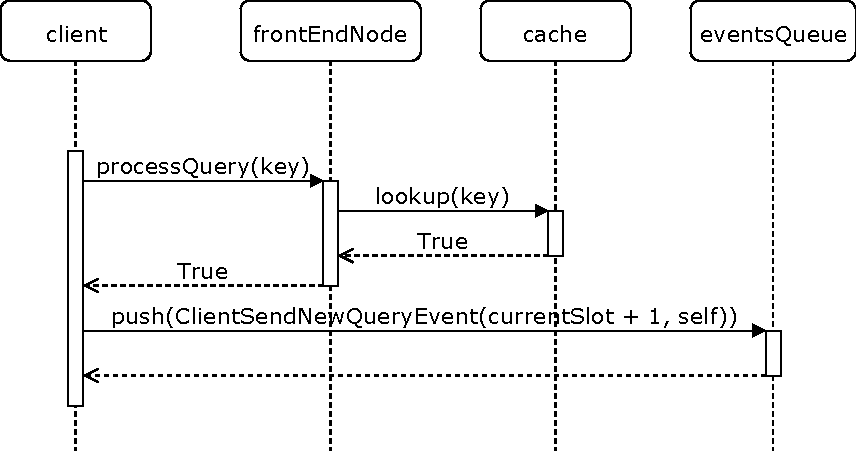
\includegraphics[scale=0.75]{img/query_hit.pdf}
	\caption{Client sends a query and the item is cached.}
	\label{fig:query_hit}
\end{figure}

\begin{figure}
	\centering
	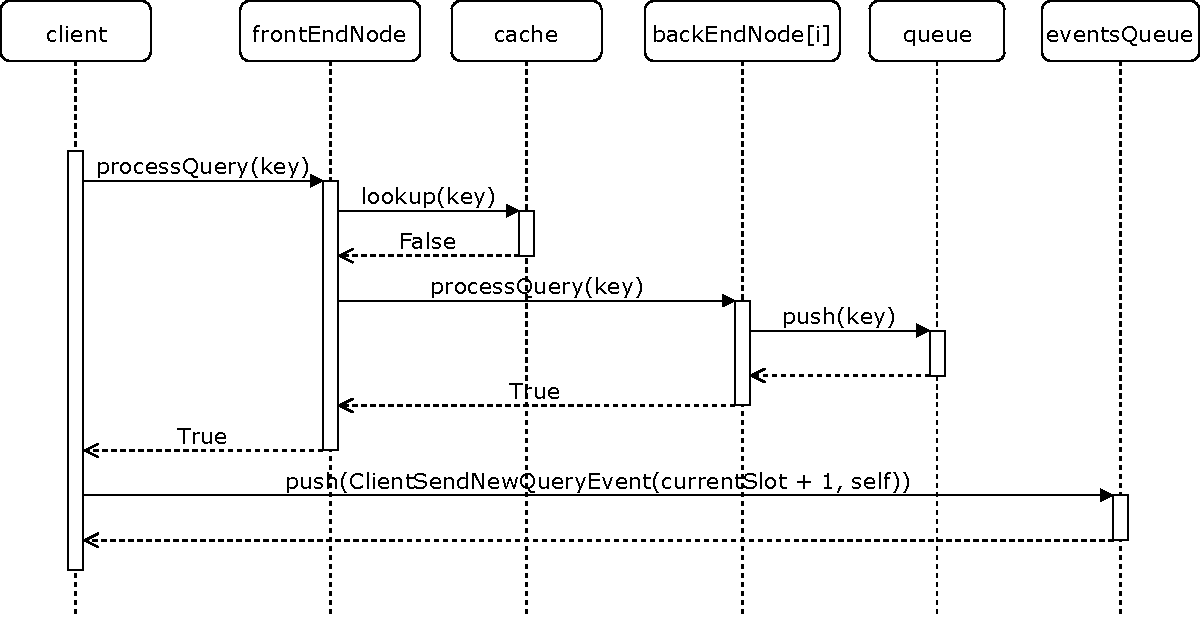
\includegraphics[scale=0.75]{img/query_miss.pdf}
	\caption{Client sends a query and the item is not cached, so it's enqueued in the back-end.}
	\label{fig:query_miss}
\end{figure}

\begin{figure}
	\centering
	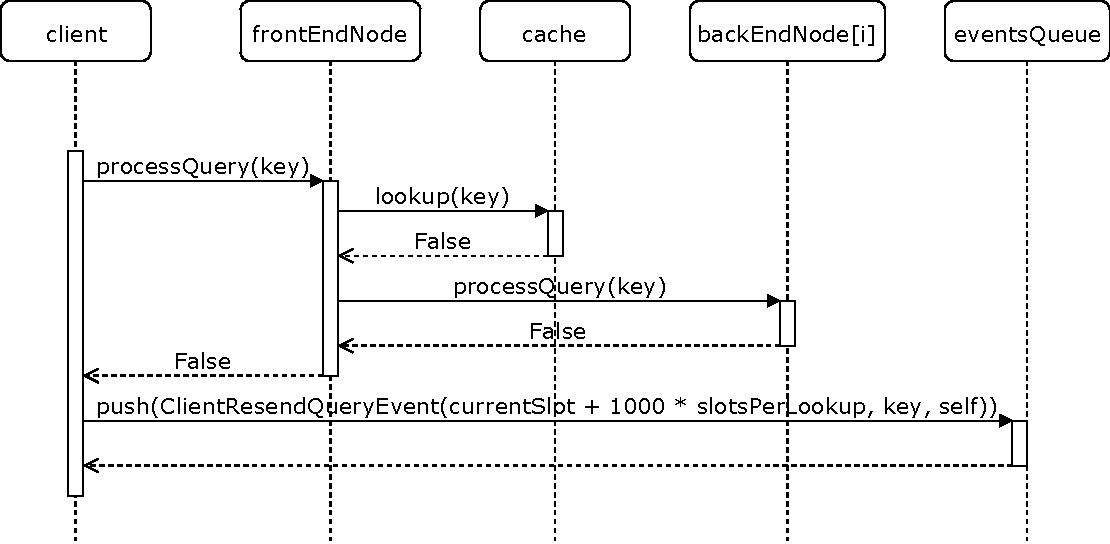
\includegraphics[scale=0.75]{img/query_full_queue.pdf}
	\caption{Client sends a query and the item is not cached, but the back-end queue is full.}
	\label{fig:query_full_queue}
\end{figure}

\begin{figure}
	\centering
	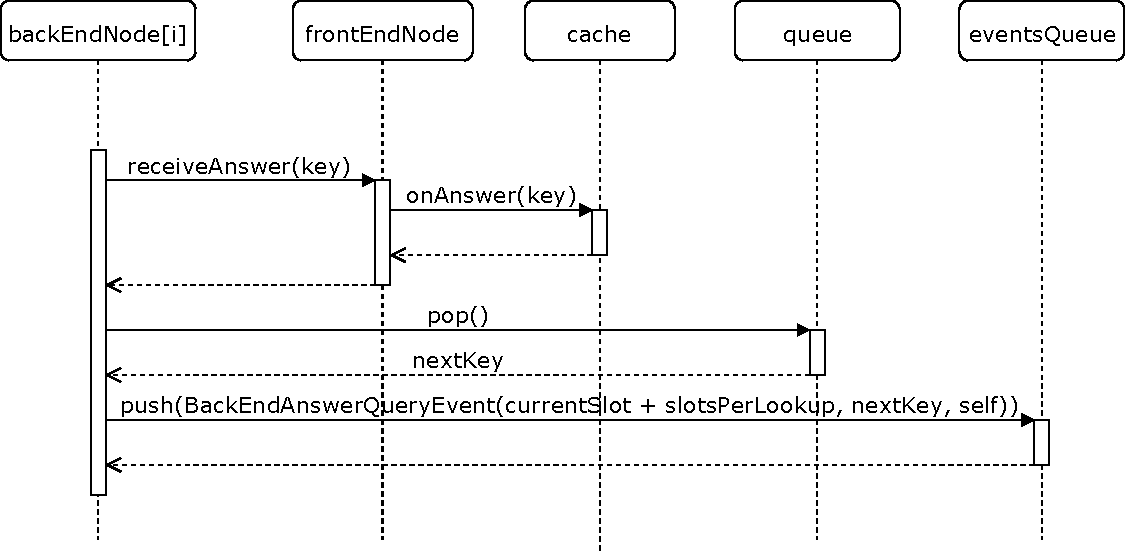
\includegraphics[scale=0.75]{img/answer_query.pdf}
	\caption{Back-end node answers a query.}
	\label{fig:answer_query}
\end{figure}

\subsection{Calibration}

Since our goal is reproducing the paper's experiments, we had to make sure our simulation setting is representative of the real-life system the authors built. In particular, our simulator could be abstracting some part of the real system which plays a non-negligible role.

We started by taking the measurements of Figure 8 in the paper (Figure \ref{fig:calibration} in our report), which shows the individual throughput of each back-end node. One would expect that given the uniformity of the adversarial strategy, queries get evenly distributed on the back-end and so should the per-machine throughput. However, since the client temporarily stops emitting requests as soon as a back-end queue gets full, a skew is introduced. When a queue gets full, the client waits until the queue gets empty to send the next query to that machine. Utilization of the congested server will be $100\%$, because it is processing queries at all times. In contrast, the remaining machines, with underfull queues, will be sitting idle waiting for the client to resume, and hence their throughput will drop.

\begin{figure}
	\centering
	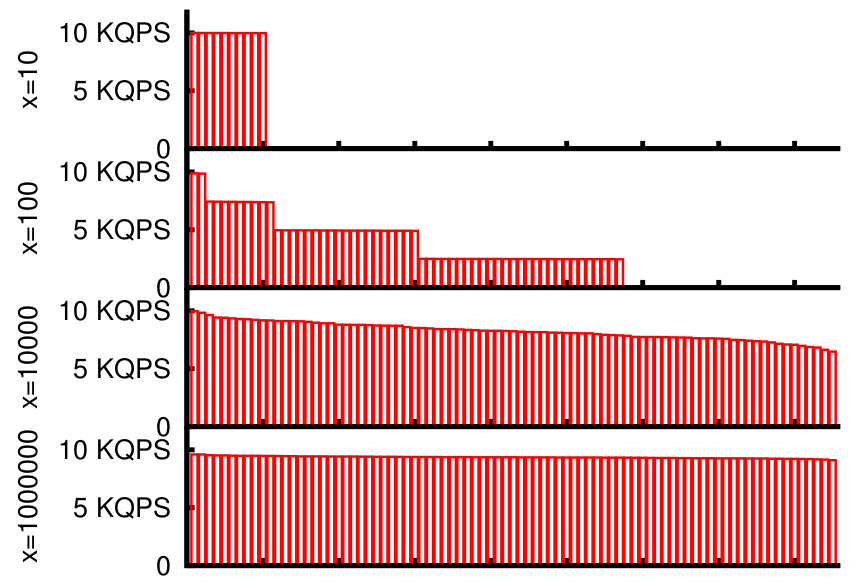
\includegraphics[scale=0.25]{img/calibration.png}
	\caption{Throughput of each back-end node for different values of $x$ (the adversarial range) when $c = 0$. Nodes are sorted according to their throughput.}
	\label{fig:calibration}
\end{figure}

Initially, our measurements didn't match with the paper's, because our first version didn't implement any kind of queuing or query rate throttling (we incorrectly underestimated this aspect). The client would continously send queries, regardless of how full a server was, which is unrealistic since servers do not have arbitrarily large buffers. After refining our simulator, we finally matched the numbers.

\section{Results and discussion}
\label{sec:results}

We attempted to replicate three experiments and obtained good results. The first experiment consists of measuring the system's throughput as a function of the adversarial range (or \textit{working set}, as called by the authors), when there is no cache. Without a cache, the worst-case scenario is an adversary that queries only one key, putting all the load on a single machine. As the adversarial range grows, the load gets distributed across all servers, so throughput increases. Our results and the paper's are shown in Figure \ref{fig:throughput_vs_working_set_no_cache}. As we can see, despite our curve is not as smooth as the paper's, the growth is similar. Discrepancies with our results are within the error ranges measured by the authors (vertical bars on each marked point), and can be attributed to features abstracted by our model. In both plots, the maximum throughput is achieved only for adversarial ranges greater than $100000$ keys, thus showing that without a cache an adversary could severely hurt performance.

\begin{figure}[h]
\centering
\begin{subfigure}[t]{.47\textwidth}
	\centering	
	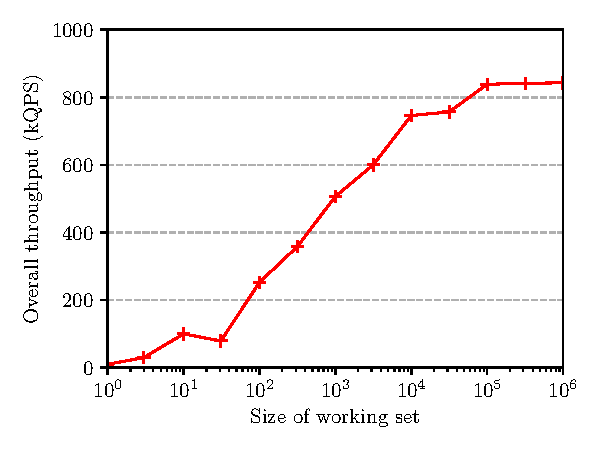
\includegraphics[scale=0.73]{img/throughput_vs_working_set_no_cache.pdf}
	\caption{Our results}
\end{subfigure}\hfill
\begin{subfigure}[t]{.47\textwidth}
	\centering
	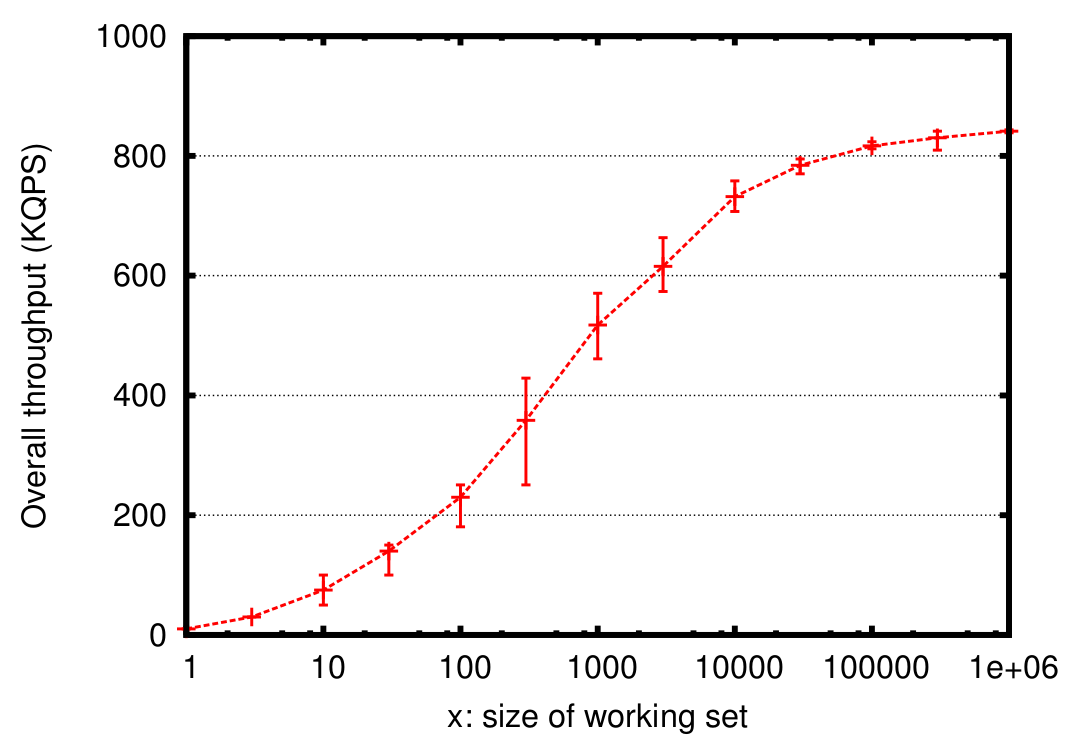
\includegraphics[scale=0.2]{img/throughput_vs_working_set_no_cache_paper.png}
	\caption{Paper's results}
\end{subfigure}
\caption{Throughput versus adversarial range, without cache (Figure 9 in the paper).}
\label{fig:throughput_vs_working_set_no_cache}
\end{figure}

The second experiment aims to learn what is the minimum cache size we need to attain maximum throughput. Specifically, we want to plot the throughput versus the cache size. The sweet spot should be about $c = k n \log n$, for a reasonable constant $k$. Figure \ref{fig:throughput_vs_cache_size} shows the results. The red curve indicates the system's throughput, whereas the blue curve is the theoretical lower bound on the system-wide achievable throughput, given by Equation \ref{eq:max_query_rate}. Since the blue curve is always below the red one, the plot corroborates Equation \ref{eq:max_query_rate}. At first sight, we can conclude that the simulation's results roughly match the paper's. A more careful examination shows that our simulation achieves maximum throughput for a cache size $1000$, whereas their measurements indicate $3000$. In any case, the order of magnitude is similar, and validates the theoretical bound. Note, however, that since the authors found the best choice to be $3000$ items, this is the cache size they used for subsequent experiments. Thus, we used $c = 3000$ as well.

\begin{figure}[h]
\centering
\begin{subfigure}[t]{.47\textwidth}
	\centering	
	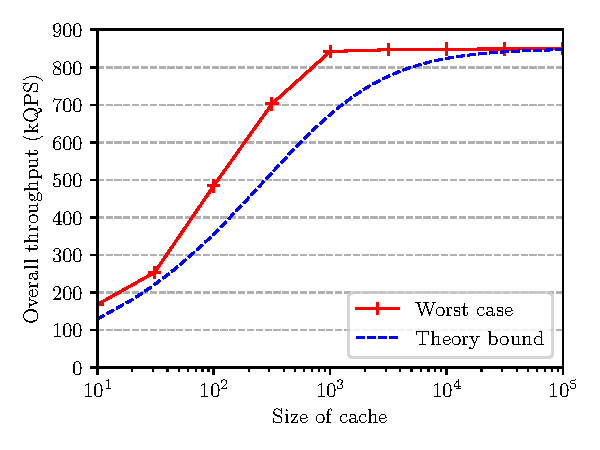
\includegraphics[scale=0.73]{img/throughput_vs_cache_size.pdf}
	\caption{Our results}
\end{subfigure}\hfill
\begin{subfigure}[t]{.47\textwidth}
	\centering
	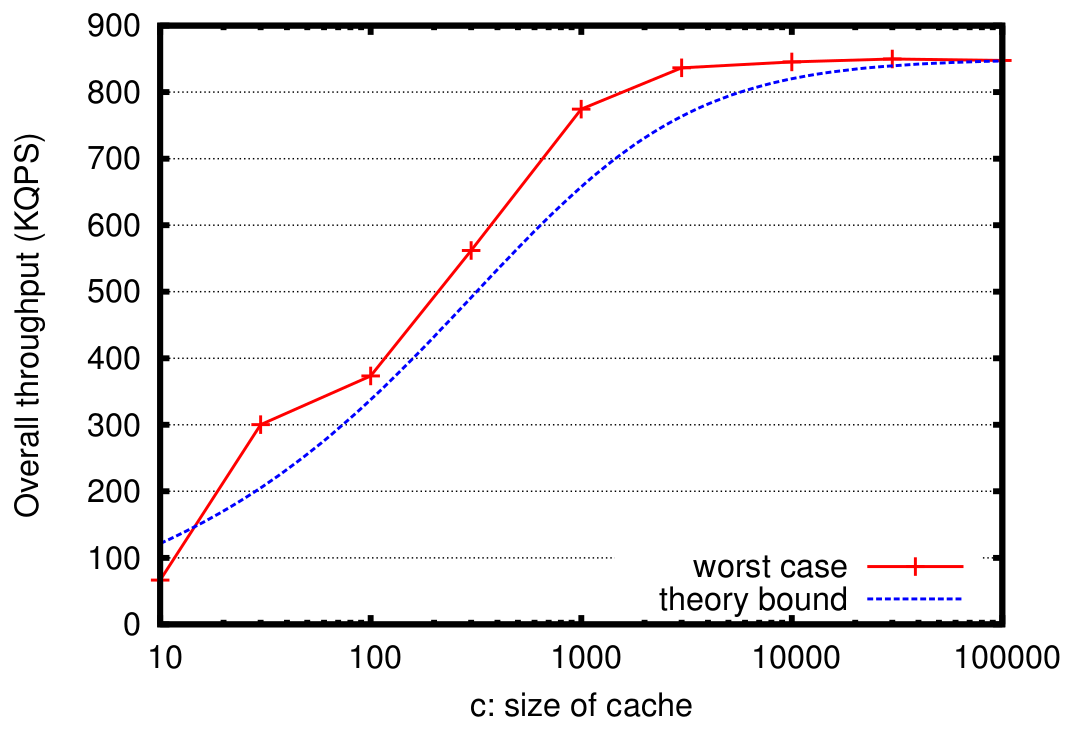
\includegraphics[scale=0.2]{img/throughput_vs_cache_size_paper.png}
	\caption{Paper's results}
\end{subfigure}
\caption{Throughput versus cache size (Figure 11 in the paper).}
\label{fig:throughput_vs_cache_size}
\end{figure}

Indeed, the third and final experiment tests the system's performance for $c = 3000$, versus several adversarial ranges. The comparison is presented in Figure \ref{fig:throughput_vs_working_set}. Again, we get similar results. The red curve shows the total throughput, which is the sum of cache and back-end throughputs. The blue line is the back-end's throughput. Since the total throughput is always greater than or close to the aggregate throughput $nt = 850$kQPS, we can conclude that such a cache allows the system to operate close to maximum utilization even under adversarial workloads. Note that at times the total throughput is over $850$kQPS. The reason is that in this experiment the query rate was set at $2nt$ (twice the back-end's capacity) to put a stressing load on the cache. Cache utilization starts at a peak (the difference between the red and blue curves is maximum), and gradually drops until both curves converge at $800$kQPS (the reason for being slightly below the aggregate throughput is, we think, related to the queuing overhead aggravated by doubling the query rate). As the adversarial range grows, cache utilization gets smaller, and the back-end starts taking care of most of the queries. Eventually, when both curves converge, the back-end is fully responsible for all the load.

\begin{figure}[h]
\centering
\begin{subfigure}[t]{.47\textwidth}
	\centering	
	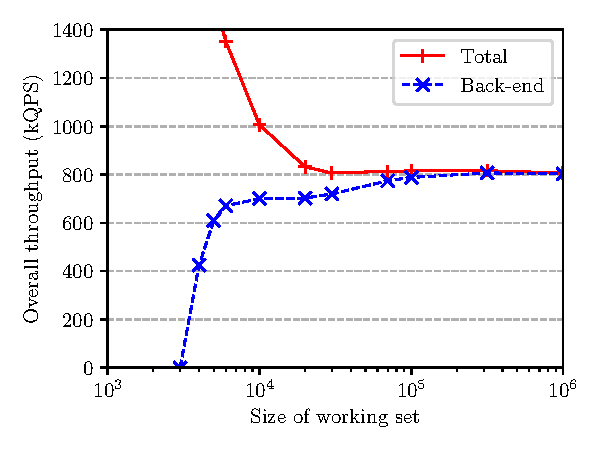
\includegraphics[scale=0.73]{img/throughput_vs_working_set.pdf}
	\caption{Our results}
\end{subfigure}\hfill
\begin{subfigure}[t]{.47\textwidth}
	\centering
	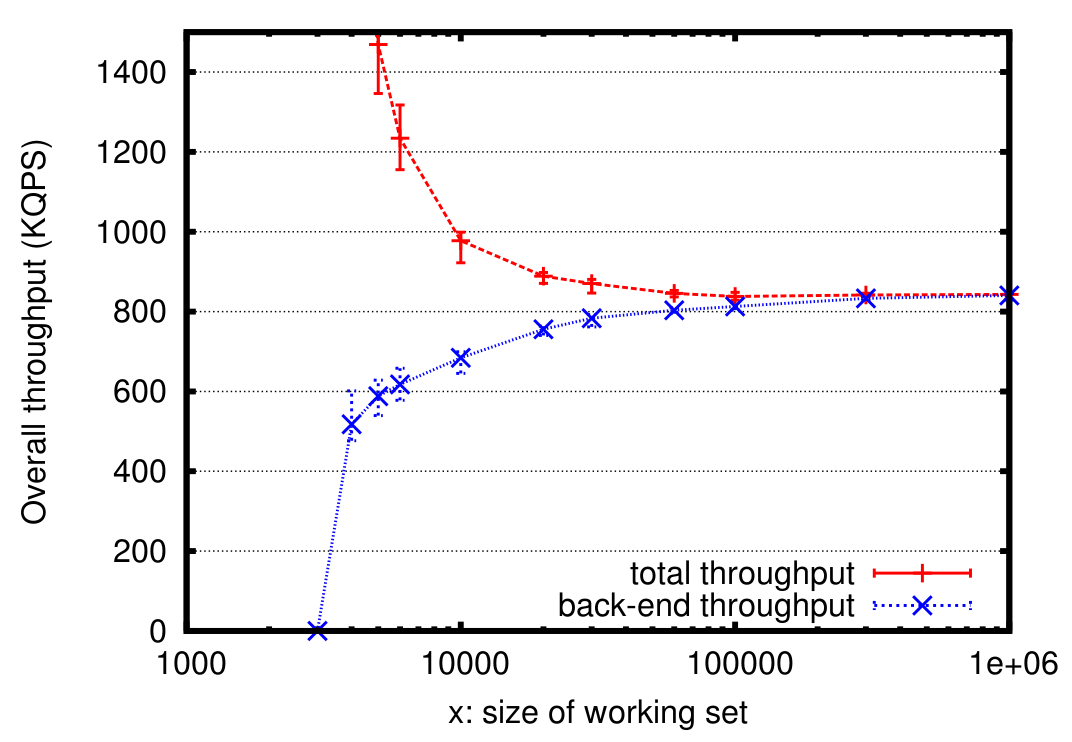
\includegraphics[scale=0.2]{img/throughput_vs_working_set_paper.png}
	\caption{Paper's results}
\end{subfigure}
\caption{Throughput versus adversarial range, with cache size $3000$ (Figure 10 in the paper).}
\label{fig:throughput_vs_working_set}
\end{figure}

\subsection{Further experimentation}

Given our relative success in replicating the authors' system and experiments, a logical follow-up is attempting to use the simulator to run further experiments and extend the paper's conclusions. This is particularly attractive, given that a simulator allows us to test arbitrarily large systems, but without the real costs of setting them up.

In particular, we wanted to test the system under a LRU caching policy, instead of a perfect cache. In this case, for a cache size $c$, an adversary will cyclically query keys $1, 2, \dots, c, c + 1$, forcing a miss for every lookup. Note that in our distributed setting cache misses do not instantly trigger an eviction followed by an insertion, because items are written after they are retrieved by the back-end. In the meantime, the client keeps issuing new queries. Thus, there might be some cache hits due to delayed evictions. However, such a cyclic pattern eventually causes cached items to be evicted at every time slot, contributing to the adversary's goal.

We repeated the experiment of Figure \ref{fig:throughput_vs_cache_size}, to see what is the minimum cache size required to achieve maximum throughput under adversarial loads, compared with the perfect cache case. The results are shown in Figure \ref{fig:throughput_vs_cache_size_lru}. The throughput in both cases is almost identical for every cache size, supporting the idea that the arguments hold for other types of caches as well.

\begin{figure}
	\centering	
	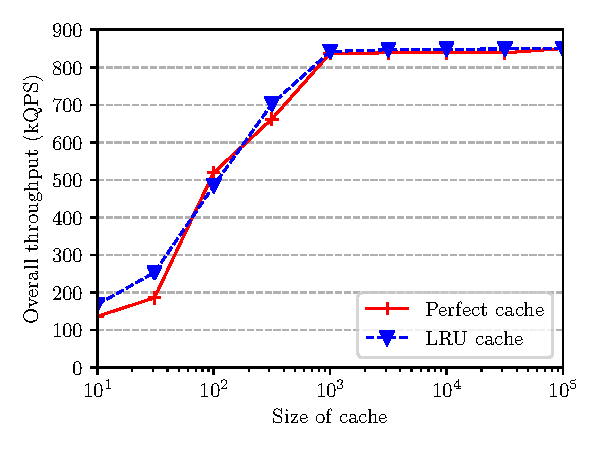
\includegraphics[scale=0.73]{img/throughput_vs_cache_size_lru.pdf}
	\caption{Throughput versus cache size, for two types of caches.}
	\label{fig:throughput_vs_cache_size_lru}
\end{figure}

\bibliographystyle{plain}
\bibliography{report}

\section{Appendix: about the software}

To run the simulation, simply execute the \texttt{run.sh} script. This will run all experiments discussed, writing results on standard output and additionally creating plots which are stored in the (automatically created) \texttt{output} folder. To change the desired set of experiments to perform, go to the main method in \texttt{simulator.py}. Each experiment has an associated flag variable that can be turned on or off.

The simulator was developed in Python, and is composed of the following files:

\begin{itemize}
	\item \texttt{cache.py}: implementations of a perfect cache, an LRU cache and adversaries.
	\item \texttt{client.py}: the client that sends queries with a particular adversarial pattern.
	\item \texttt{events.py}: the events queue and the different types of events that can happen.
	\item \texttt{nodes.py}: front-end and back-end nodes.
	\item \texttt{plot.py}: a helper class to plot experiment results.
	\item \texttt{simulator.py}: the simulator and several hardcoded experiments.
	\item \texttt{stats.py}: simulation metrics and statistics.
\end{itemize}

\end{document}